\documentclass{article}
\usepackage{tikz}
\usepackage{pgfplots}
\pgfplotsset{compat=newest}
\usepackage{mathtools}
\usepackage{amssymb}

\begin{document}

$ A=\{(x,y) \in \mathbb{R}^2 : x^2 + y^2 <1 \} $

$ B=\{(x,y) \in \mathbb{R}^2 : y \leq x  \} $\\

A sketch of $ A \cap B $\\

        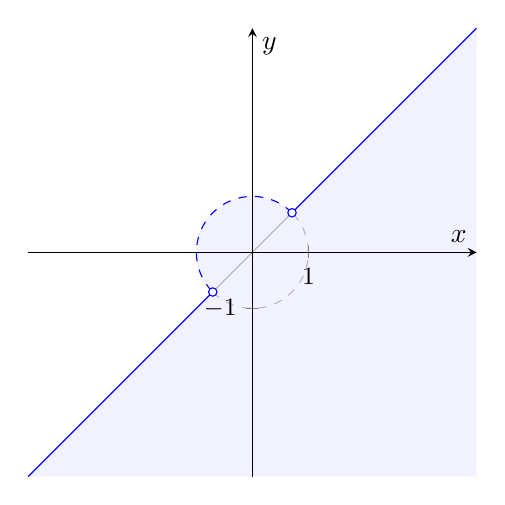
\begin{tikzpicture}
            \begin{axis}[xmin=-4, xmax=4, ymin=-4, ymax=4,axis equal image,axis lines=none]
                
                \fill [opacity=0.05,fill=blue, domain=-4:4]
                (axis cs:4,-4)
                -- plot (\x,\x)
                -- cycle;
        
                
                \draw [blue, opacity=0.05,fill=blue,dashed](axis cs:0.7071,0.7071) arc[radius =1, start angle= 45, end angle= 225];
                \draw [blue, dashed](axis cs:0.7071,0.7071) arc[radius =1, start angle= 45, end angle= 225];
                \draw [gray,opacity=0.5, dashed](axis cs:-0.7071,-0.7071) arc[radius =1, start angle= 225, end angle= 405];
                    
                \addplot [blue][mark=none,domain=-4:-0.7071] {x};
                \addplot [blue][mark=none,domain=0.7071:4] {x};
                \addplot [gray,opacity=0.5][mark=none,domain=-0.7071:0.7071] {x};
                \draw [blue, fill=white] (axis cs:0.7071,0.7071) circle (0.075) ;
                \draw [blue, fill=white] (axis cs:-0.7071,-0.7071) circle (0.075) ;
                        
            \end{axis}
        
 
            \begin{axis}[
            axis lines = middle,
            axis equal image,
            xlabel={ $x$},
            ylabel={$y$},
            xtick={1},
            ytick={-1},
            xticklabel ={\small $ 1 $},
            yticklabel ={\small $ -1 $},
            xmin=-4, xmax=4, ymin=-4, ymax=4,
            ]
            \end{axis}
        \end{tikzpicture}\\
        A sketch of $  B-A $\\
        
        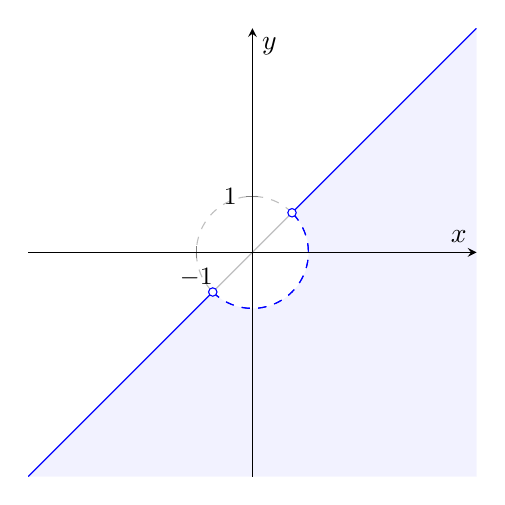
\begin{tikzpicture}
        \begin{axis}[xmin=-4, xmax=4, ymin=-4, ymax=4,axis equal image,axis lines=none]
        
        \fill [opacity=0.05,fill=blue, domain=-4:4]
        (axis cs:4,-4)
        -- plot (\x,\x)
        -- cycle;
        
        
        \draw [blue, dashed, fill=white](axis cs:-0.7071,-0.7071) arc[radius =1, start angle= 225, end angle=405];
        \draw [gray,opacity=0.5, dashed](axis cs:0.7071,0.7071) arc[radius =1, start angle= 45, end angle= 225];
        \draw [blue, dashed](axis cs:-0.7071,-0.7071) arc[radius =1, start angle= 225, end angle= 405];
        
        \addplot [blue][mark=none,domain=-4:-0.7071] {x};
        \addplot [blue][mark=none,domain=0.7071:4] {x};
        \addplot [gray,opacity=0.5][mark=none,domain=-0.7071:0.7071] {x};
        \draw [blue, fill=white] (axis cs:0.7071,0.7071) circle (0.075) ;
        \draw [blue, fill=white] (axis cs:-0.7071,-0.7071) circle (0.075) ;
        
        \end{axis}
        

        \begin{axis}[
        axis lines = middle,
        axis equal image,
        xlabel={ $x$},
        ylabel={$y$},
        xtick={-1},
        ytick={1},
        xticklabel ={\small $ -1 $},
        yticklabel ={\small $ 1 $},
        xmin=-4, xmax=4, ymin=-4, ymax=4,
        ]
        \end{axis}
        \end{tikzpicture}


\end{document}
